\chapter{Integrating dimensions of prosody}
\label{chapter_multi_prosody}

The analysis of the current corpus of prosodic focus marking so far has concentrated on modulations of parameters related to F0. It was, however, shown in Chapter \ref{chapter_prosody} that modifications of the supra-laryngeal articulatory subsystem play an important role in prosodic prominence as well \citep{Cho2011, Mücke2018}. This chapter extends the analysis of the corpus to include tongue body and lip movements. In doing so, evidence will be provided that prosodic prominence can be regarded as a multi-dimensional bundle. The chapter also aims to gain a deeper insight into the tonal patterns of prosodic marking of focus by looking at unaccented tokens.

The modelling approach outlined in the previous chapter (Chapter \ref{chapter_onglide_modelling}) is enriched in a two-fold manner: First, the consequences of accent placement are integrated in the model. This is achieved by proposing a property of the model that results in a bifurcation, i.e. a qualitative change, when the control parameter is changed past a certain threshold. Second, the articulatory dimensions are included in the model, employing the same control parameter for F0 and articulatory patterns.

\section{Results of F0 measures}

The previous chapter (Chapter \ref{chapter_onglide_modelling}) presented the results of the tonal onglide measure that revealed the categorical and continuous nature of prosodic parameters at the same time. The analysis there was restricted to the nuclear pitch accents. However, focussing on nuclear pitch accents exclusively leaves an important part of the data aside, namely the condition in which the target word is in background. As described in Chapter \ref{chapter_data}, an equivalent measure of tonal onglide was performed on these unaccented cases using fixed time points (5 ms before the start and 50 ms before the end of the stressed syllable). This measure is employed in what follows to add the missing piece to the picture and to extend the model.

Before turning to the quantitative results, an example of a contour with an early nuclear accent on the direct object is presented to give a better impression of the kind of data that are analysed. As Figure \ref{fig:contour_background} illustrates for one production of a male speaker (the same male speaker as in the contours in \ref{fig:example_contours}), not placing an accent on the target word yields a flat stretch of F0 on and around the target word. 

\begin{figure}[t]
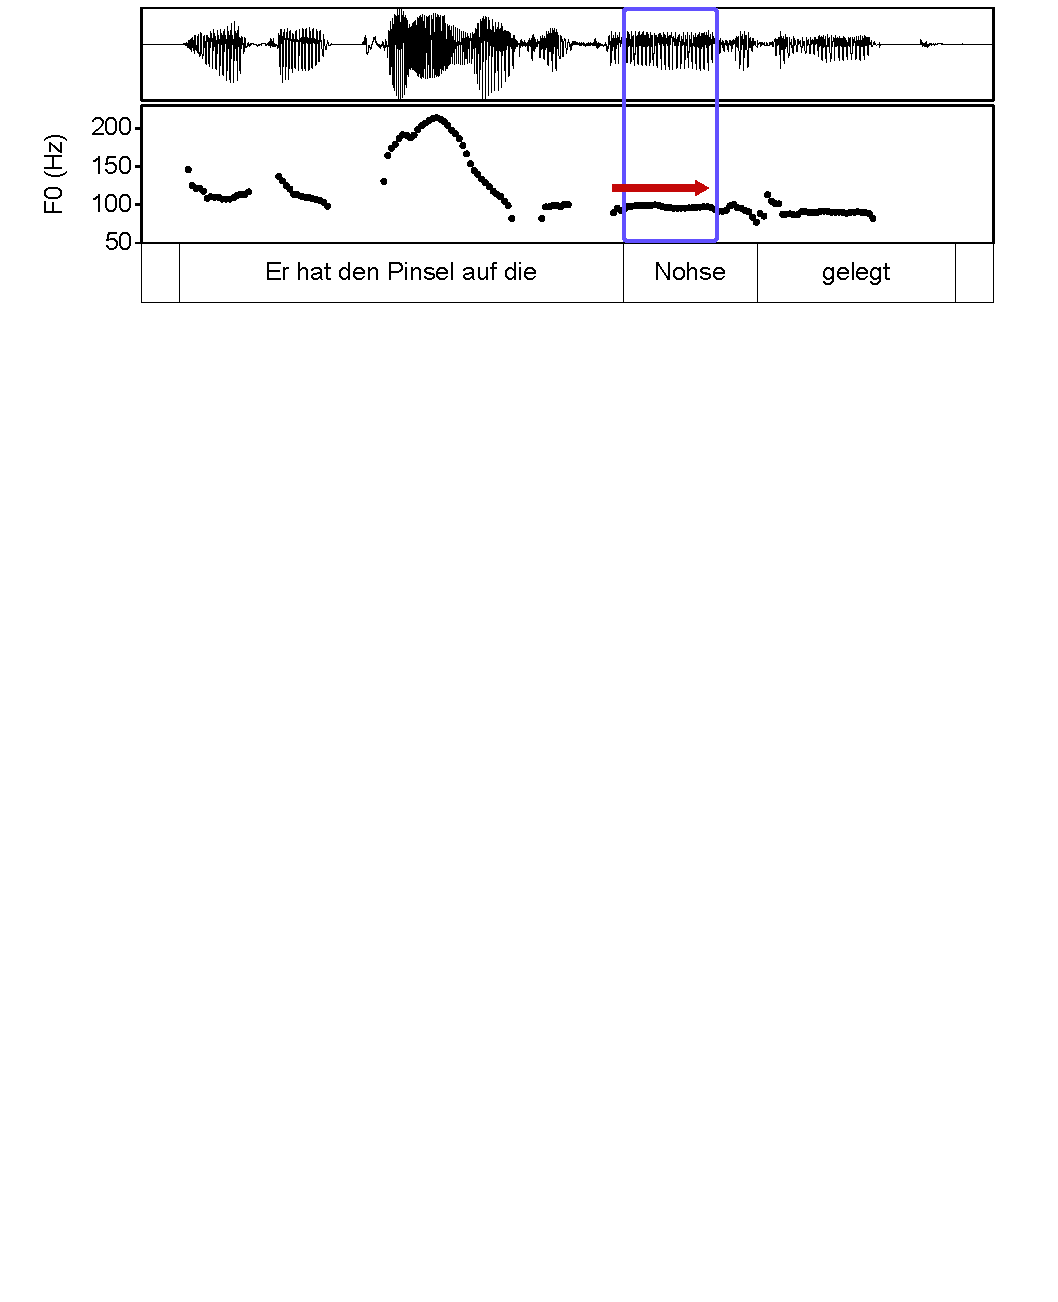
\includegraphics[width=\textwidth]{figures/ch7/intonation_contour_background.pdf}
\caption[Example intonation contour for the background condition.]{Example intonation contour for the background condition. The blue box indicates the lexically stressed (but unaccented) syllable of the target word. The red arrow traces the tonal onglide equivalent.}
\label{fig:contour_background}
\end{figure}

The fact that the F0 contour is flat on unaccented target words is reflected in the distributions of the tonal onglide displayed in Figure \ref{fig:onglide_distributions_across}. The distribution for background is characterised by a single mode slightly below zero. The other three conditions (broad focus, narrow focus, contrastive focus) are as reported in Chapter \ref{chapter_onglide_modelling} but are repeated here to be able to compare their distributions to the background condition. Repeated for convenience here are also the means of the rising accents, see Figure \ref{fig:onglide_means_second_occurence}. This figure only includes broad focus, narrow focus and contrastive focus since it is only possible to speak of rises in these cases. 

In sum, the full analysis of the tonal onglide reveals the following picture: In the background condition, the data show a single mode located slightly below zero. For broad focus, a bimodal shape of the distribution can be observed, with almost equal numbers of falling and rising onglides. In narrow and contrastive focus, the right mode is more pronounced (more rises in narrow compared to broad focus, and more rises in contrastive compared to narrow focus). In addition to the increase in the number of accents with a rising onglide, the magnitude of the onglides becomes larger, as reflected in the stepwise growth of the mean from broad focus to narrow focus, and from narrow focus to contrastive focus. The next section attempts to capture this pattern with a dynamical description.

\begin{figure}
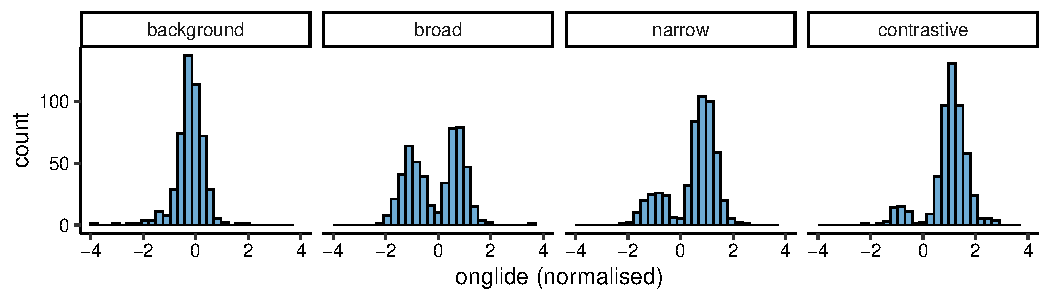
\includegraphics[width=\textwidth]{figures/ch7/onglide_norm_distribution_all.pdf}
\caption{Distributions of normalised tonal onglide values for background, broad, narrow and contrastive focus.}
\label{fig:onglide_distributions_across}
\end{figure}

\begin{figure}
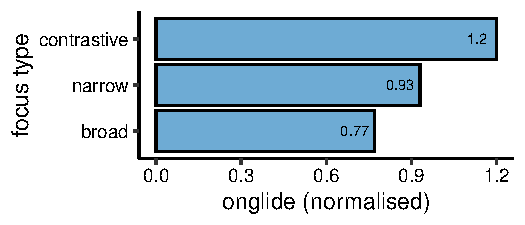
\includegraphics[width=7.5cm]{figures/ch7/onglide_norm_rising_means.pdf}
\caption{Means of rising onglides (normalised) for broad, narrow and contrastive focus.}
\label{fig:onglide_means_second_occurence}
\end{figure}

\section{Enriching the tonal onglide model I: accentuation}

This section is concerned with the development of a model to account for the results outlined above. In order to be able to exhibit a behaviour that is consistent with the data, the model sought here needs to change from a monostable attractor landscape to a bistable attractor landscape when moving from background to broad focus (first pattern of behaviour). In addition, the attractor landscape needs to be able to tilt to one or the other side giving more stability to one of the attractors (second pattern of behaviour). Both types of changes need to be induced by the scaling of a control parameter.

The first pattern of behaviour can be obtained by a model like the one described by the potential $A(x) = \frac{x^4}{4} - kx^2$ as displayed in the upper row of Figure \ref{fig:example_models} for different values of the control parameter $k$. When $k$ is below zero, the system has only one attractor. When $k$ passes zero, the system's landscape develops into a landscape with two attractors. The second pattern of behaviour is exhibited by a model like the one described by the potential $B(x) = \frac{x^4}{4} - x^2 - kx$. This is a version of the typical double-well potential that was discussed several times in the course of this book and is also used in the modelling of the tonal onglide in the previous chapter (Chapter \ref{chapter_onglide_modelling}). This landscape tilts from left to right when $k$ is scaled from negative to positive values.

\begin{figure}
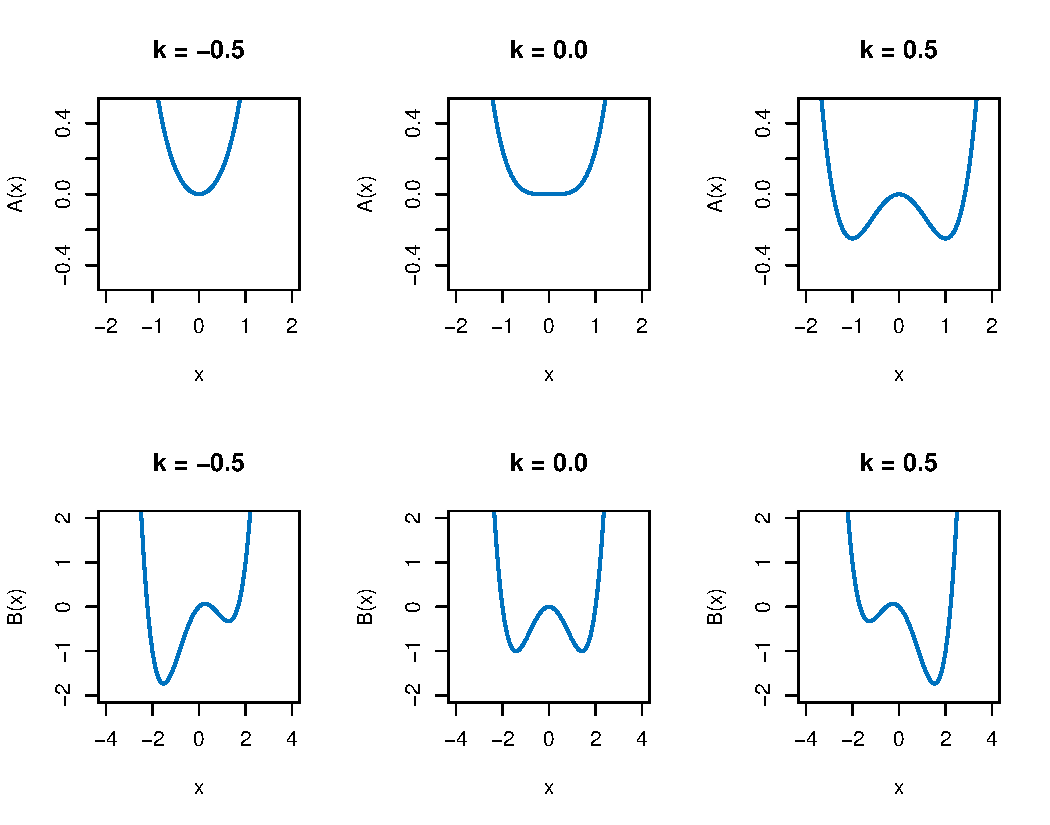
\includegraphics[width=\textwidth]{figures/ch7/example_models.pdf}
\caption[Example models $A(x)$ and $B(x)$.]{Example models $A(x)$ (top) and $B(x)$ (bottom) for different control parameter $k$ values.}
\label{fig:example_models}
\end{figure}

\newpage
A possible model that ties these two patterns together can be formulated as given in Equation \ref{eq:onglide_model2} by the potential $V(x)$ and the corresponding force $F(x)$. Choosing parameter values for background, broad focus, narrow focus and contrastive focus, one can observe the change in the system as shown in Figure \ref{fig:potentials_force_bg_br_na_co}. The attractor landscape is monostable for $k = -0.5$ (background) but is bistable for $k = 2.1$ (broad focus). Scaling the control parameter further tilts the landscapes to the right side (i.e. it stabilises the rising attractor) for $k = 2.5$ (narrow focus) and $k = 3.0$ (contrastive focus). The jump from background to broad focus appears large. It has to be borne in mind, however, that the system has to go through a stage where the falling accents dominate the system's outcome. In this stage, the left attractor has to be more stable, e.g. to model the results of speaker group 1 (see Chapter \ref{chapter_onglide_modelling}).

\begin{equation}
\begin{split}
V(x) = \frac{x^4}{4} - (1-e^{\frac{1}{2}-k})x^2 - \frac{|k|(k-2)x}{4} \\
F(x) = - x^3 + 2(1-e^{\frac{1}{2}-k})x + \frac{|k|(k-2)}{4}
\label{eq:onglide_model2}
\end{split}
\end{equation}

\begin{figure}
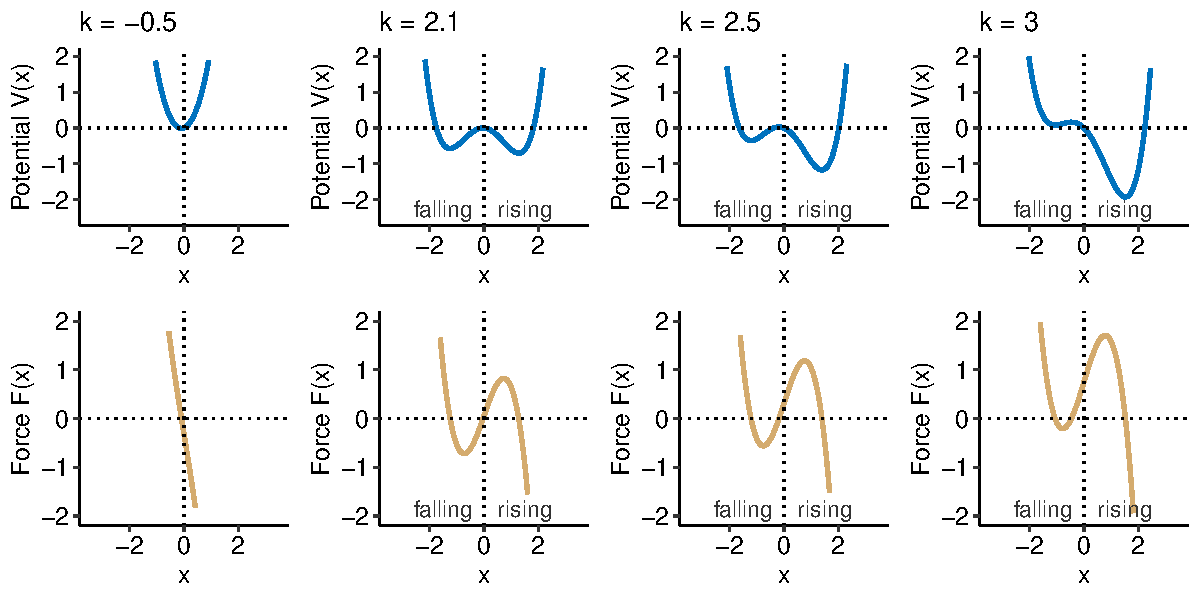
\includegraphics[width=\textwidth]{figures/ch7/potentials_force_model2.pdf}
\caption{Potential and force functions for $k$ values modelling background ($k=-0.5$), broad ($k=2.1$), narrow ($k=2.5$) and contrastive focus ($k=3$).}
\label{fig:potentials_force_bg_br_na_co}
\end{figure}

Using a simulation with the addition of noise, the outcome of the model as a stochastic system can be observed; see Figure \ref{fig:simulation_bg_br_na_co} (distributions) and Figure \ref{fig:simulation_means_bg_br_na_co} (means for accented focus types). The simulation works as described before in Chapter \ref{chapter_onglide_modelling}. The differential function describing the system (the force function) is solved using small discrete time steps in each of which noise is added in the form of a random number from a Gaussian distribution with a mean of $0$ and standard deviation of $0.03$. The simulation is finished after 5,000 time steps and records the solution. In total, 2500 solutions are recorded.

The same characteristic pattern as in the results for the tonal onglide can be attested: The system produces a unimodal distribution slightly below zero for background. The bimodal distribution of broad focus is nearly symmetrical. In narrow and contrastive focus, the right mode (rising) becomes increasingly strong. The mean values of the rising (positive) distributions also show essentially the same stepwise increase for the “accented” focus types (broad, narrow and contrastive focus). This result reveals that the rising (right) attractor moves toward more extreme values when the control parameter value is increased and the attractor landscape tilts to the right side.

\begin{figure}[t]
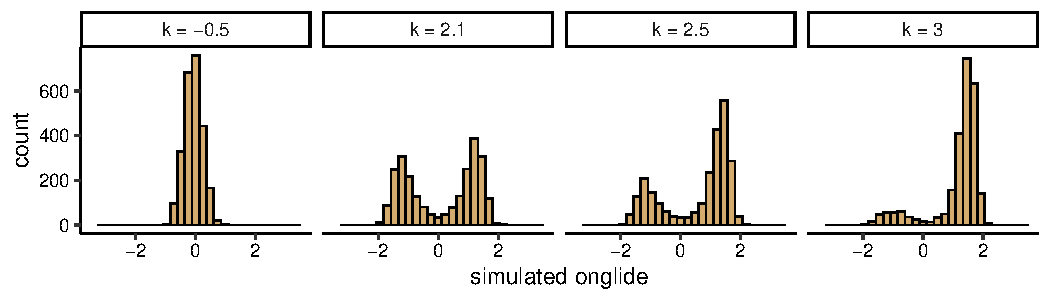
\includegraphics[width=\textwidth]{figures/ch7/onglide_all_across.pdf}
\caption{Distributions of simulation results for $k$ values modelling background ($k=-0.5$), broad ($k=2.1$), narrow ($k=2.5$) and contrastive focus ($k=3$).}
\label{fig:simulation_bg_br_na_co}
\end{figure}

\begin{figure}[t]
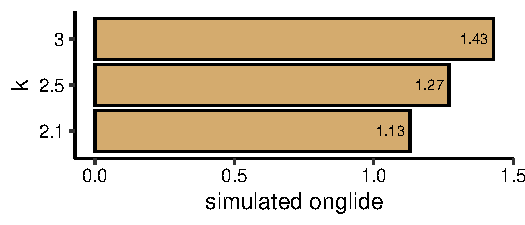
\includegraphics[width=7.5cm]{figures/ch7/positive_means_across.pdf}
\caption{Means of positive simulated onglides for $k$ values modelling broad ($k=2.1$), narrow ($k=2.5$) and contrastive focus ($k=3$).}
\label{fig:simulation_means_bg_br_na_co}
\end{figure}

The proposed model captures the main features of the tonal onglide data and produces a close qualitative correspondence to the empirical data. The change from background to broad focus is modelled with a bifurcation from monostable to bistable. The modifications from broad to narrow focus, and from narrow to contrastive focus are modelled with the tilt of the bistable landscape. Crucially, all this happens as the consequence of scaling the same parameter.

\section{Results of articulatory measures}

F0 has been shown to be a very important parameter in signalling prosodic prominence and modulating the signal in order to encode pragmatic meanings. However, the literature has accumulated numerous examples of modifications of the supra-laryngeal articulation going hand in hand with prosodic structure \citep[for overviews see][]{Cho2011, Mücke2018}. This section is concerned with the exploration of lip and tongue movements in the data set. The data set does not contain missing values (NA) for the articulatory parameters. Hence, of the 2088 rows of the complete data set, all data points can be used. One half (1044 data points) contains data for the target words with vowel /a/, the other half contains data for the target words with /o/. All values of the articulatory measures presented here are z-scored for speaker and vowel.

Figure \ref{fig:eukl_max} presents the distributions and means of the maximal lip aperture during the opening of the vowel in the stressed syllable for both /a/ and /o/ and the four focus conditions. Although -- as an inspection of the distributions reveals -- the modifications are rather subtle, there is a systematic trend for the lips to be opened wider in broad focus compared to background, in narrow focus compared to broad focus, and in contrastive focus compared to narrow focus, or put more succinctly: background < broad focus < narrow focus < contrastive focus. This trend appears to be more pronounced in the vowel /a/ compared to /o/.

In light of the literature on prosodic strengthening, the opening of the lips to convey higher levels of prominence is interpreted as \emph{sonority expansion}. Employing this strategy the speaker aims to increase the acoustic energy radiating from the mouth \citep{BeckmanEdwardsFletcher1992}. In the case of the low vowel /a/, the higher degree of lip opening could also be a concomitant of a lower jaw position. The lower jaw position would allow for a lower tongue position to be employed as \emph{localised hyperarticulation} of the low vowel \citep{DeJong1995}. In either case, it is important to note that the prosody-induced modification of the articulatory gestures that are responsible for lip aperture does not only occur between unaccented and accented (i.e. background vs. broad focus) but also within the group of focus types that all share the same nuclear pitch accent location (i.e. the accent remains on the target word in broad, narrow and contrastive focus).

\begin{figure}
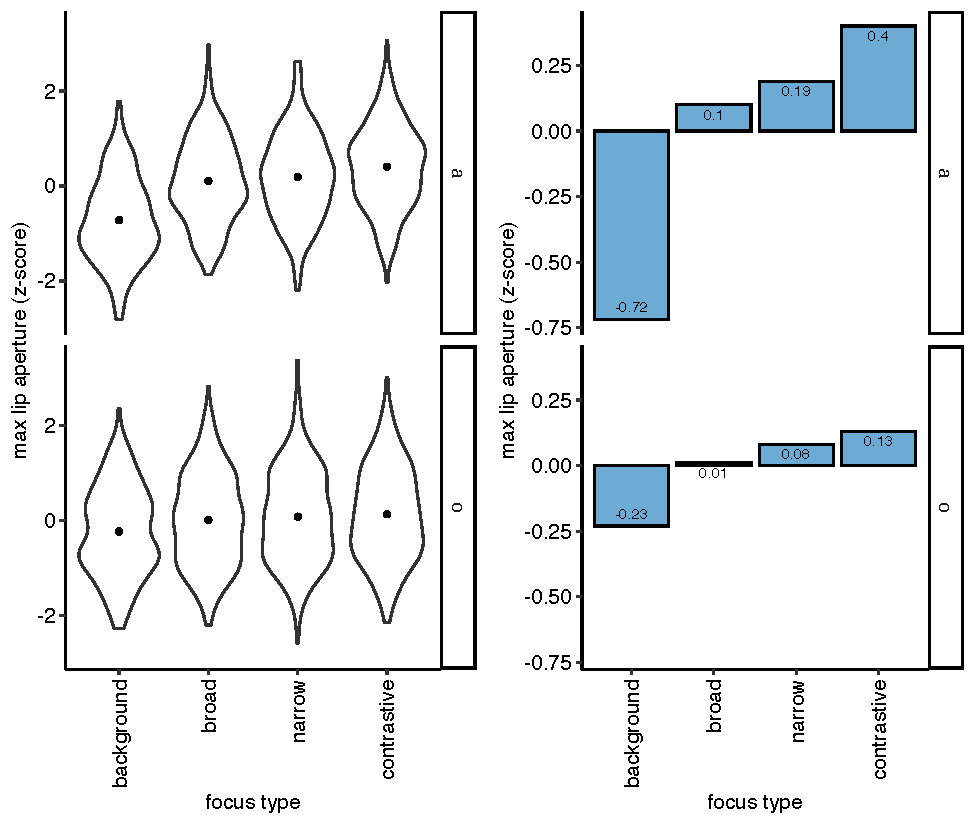
\includegraphics[width=\textwidth]{figures/ch7/eukl_max.pdf}
\caption[Distributions and mean values of the maximal lip aperture.]{Distributions (left) and mean values (right) of the maximal lip aperture for /a/ (top) and /o/ (bottom). The black dots in the distributions on the left indicate the position of the means for comparison with the right panel.}
\label{fig:eukl_max}
\end{figure}

Figure \ref{fig:tboy} illustrates the results of the vertical tongue body position, extracted using the 50\% window method, in distributions and means for both vowels and all focus types. As in the case of lip aperture, the differences between focus types seem to be subtle but systematic: The tongue body position is lowered in both /a/ and /o/ from background to broad focus, from broad focus to narrow focus, and from narrow focus to contrastive focus: background > broad focus > narrow focus > contrastive focus.\footnote{The direction is reversed since the tongue body is lowered and the values therefore decrease.}



For the low vowel /a/, this trend can again be identified as localised hyperarticulation and sonority expansion at the same time. On the one hand, a lower tongue body strengthens the identity of the low vowel. On the other hand, a lower jaw, used to let more acoustic energy radiate from the mouth, may also lead to a lower tongue body position. For the mid vowel /o/, the interpretation as sonority expansion seems more plausible. Again, the modifications do not exclusively take place under the influence of accentuation (i.e. from background to broad) but also within the group of accented target words to mark different focus types (broad $\,\to\,$ narrow $\,\to\,$ contrastive focus).

\begin{figure}
	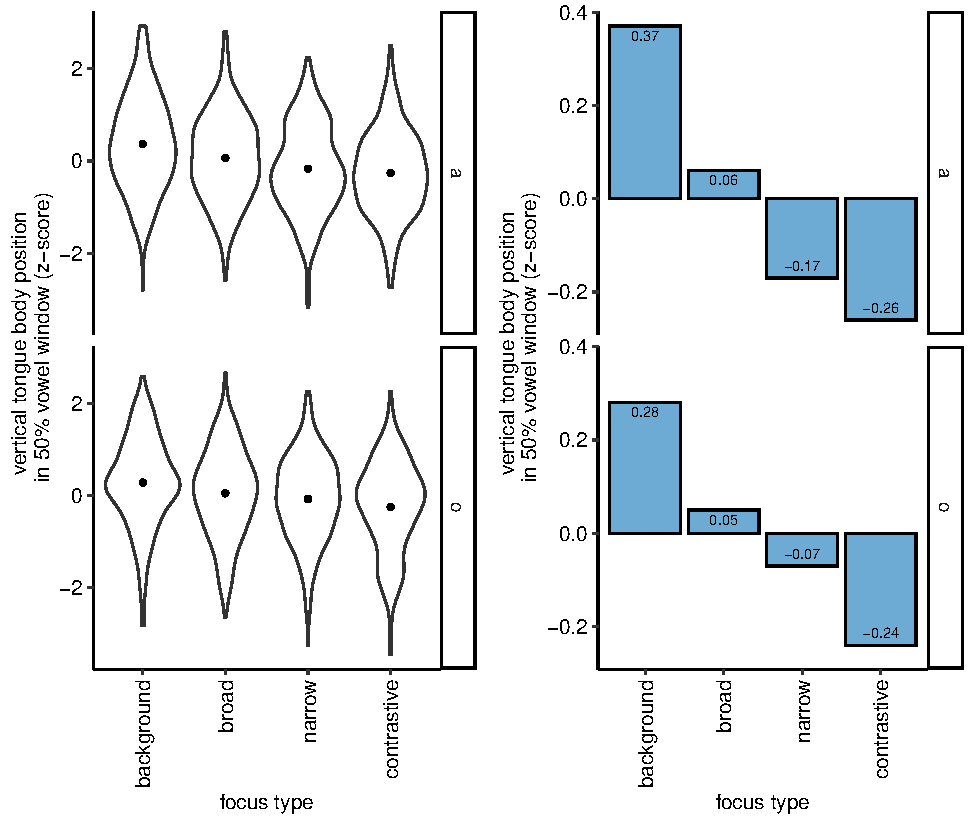
\includegraphics[width=\textwidth]{figures/ch7/tboy.pdf}
	\caption[Distributions and mean values of the vertical tongue body position.]{Distributions (left) and mean values (right) of the vertical tongue body position for /a/ (top) and /o/ (bottom). The black dots in the distributions on the left indicate the position of the means for comparison with the right panel.}
	\label{fig:tboy}
\end{figure}


Finally, Figure \ref{fig:tbox} shows the distributions and means for the horizontal tongue body position for both vowels and all focus types, extracted using the 50\% window method. The results for /a/ do not show the clear trend found in the other parameters. In addition, the differences seem to be rather small. For the vowel /a/, hence, no conclusive results can be obtained for the horizontal tongue position. In contrast, for the vowel /o/, the trend observed in the other parameters is present. The tongue body is retracted from background to broad focus, from broad focus to narrow focus and from narrow focus to contrastive focus. These results are indicative for localised hyperarticulation of the back vowel /o/. 

\begin{figure}
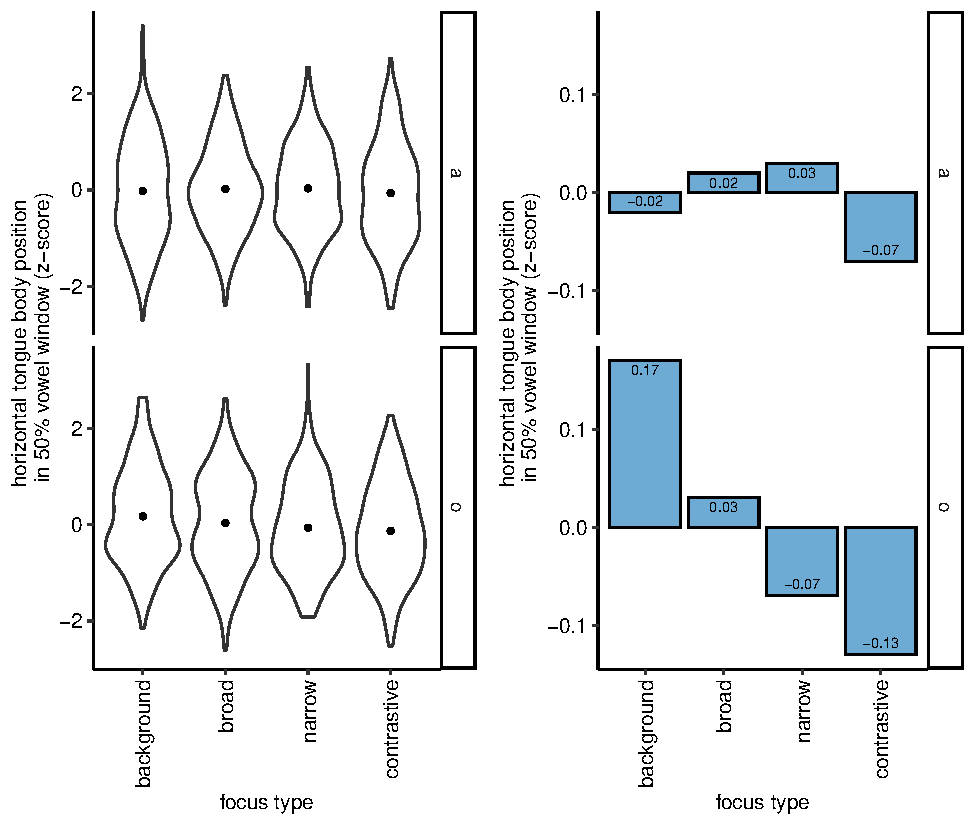
\includegraphics[width=\textwidth]{figures/ch7/tbox.pdf}
\caption[Distributions and mean values of the horizontal tongue body position.]{Distributions (left) and mean values (right) of the horizontal tongue body position for /a/ (top) and /o/ (bottom). The black dots in the distributions on the left indicate the position of the means for comparison with the right panel.}
\label{fig:tbox}
\end{figure}

Analogously to the tonal onglide analysis in the previous chapter (Chapter \ref{chapter_onglide_modelling}), the results are analysed using Bayesian linear mixed models in R \citep{RCoreTeam2018} with the package brms \citep{Buerkner2018}. The estimated differences between focus conditions in terms of posterior means are reported in addition to 95\% credible intervals. Given the data and the model, the 95\% credible intervals indicate the range in which one can be certain with a probability of 0.95 that the difference between estimates can be found. To calculate the differences between focus types, the analysis subtracts the posterior samples for background from broad focus (broad–background), broad focus from narrow focus (narrow–broad), narrow focus from contrastive focus (contrastive–narrow), and broad focus from contrastive focus (contrastive–broad). 

In the case of the maximal lip aperture, the probability of the estimate being greater than zero is reported because it is interesting whether the lip aperture increases from one focus type to another. In the case of the tongue position measures, the probability of the difference being smaller than zero is reported, because it is interesting  whether the tongue position is lower or more retracted, i.e. whether the values decrease, from one focus type to another. All models are run separately for each vowel (/a/ or /o/).

The models include one z-scored articulatory parameter each (maximal lip aperture, vertical tongue position, horizontal tongue position) as the dependent variable. In all models, focus type is a fixed effect, and random intercepts for speakers and target words as well as by-speaker and by-target word slopes for the effect of focus type are included. The priors are centred around zero, the models run with four sampling chains of 3,000 iterations each.

The presentation starts with the modelling results for the maximal lip aperture for the vowel /a/. Given the model and the data, the analysis yields a clear difference in the posterior probabilities between background and broad focus ($\hat\beta=0.81 , \text{CI}=[0.65, 0.97], \allowbreak Pr(\hat\beta>0)=1$) and broad and contrastive focus ($\hat\beta=0.30 , \text{CI}=[0.12, 0.49], \allowbreak Pr(\hat\beta>0)=1$), i.e. across accentuation (background vs. broad) as well as within accentuation (broad vs. contrastive focus). There is also clear evidence for differences between narrow and contrastive focus ($\hat\beta=0.21 , \text{CI}=[0.02, 0.40], \allowbreak Pr(\hat\beta>0)=0.99$), while the evidence is not as strong for the opposition of broad vs. narrow focus ($\hat\beta=0.09 , \text{CI}=\allowbreak[-0.08, 0.26], \allowbreak Pr(\hat\beta>0)=0.84$).

For the vowel /o/, the model shows evidence for differences between background and broad ($\hat\beta=0.24 , \text{CI}=[0.08, 0.39], \allowbreak Pr(\hat\beta>0)=1$). There is weaker evidence for a difference between broad and contrastive ($\hat\beta=0.12, \text{CI}=[-0.05, 0.30], \allowbreak Pr(\hat\beta>0)=0.92$). Narrow focus seems to pattern with contrastive focus, but there is no clear evidence for narrow focus to be differentiated from broad ($\hat\beta=0.07 , \text{CI}=[-0.11, 0.23], \allowbreak Pr(\hat\beta>0)=0.79$) or contrastive ($\hat\beta=0.05, \text{CI}=[-0.12, \allowbreak 0.23], \allowbreak Pr(\hat\beta>0)=0.73$). 

To sum up the results of the lip aperture: Modifications of the degree of lip opening are attested from unaccented to accented (background < broad focus) and also within the group of accented focus types (broad < contrastive focus). The modifications always go in the same direction, the lips are opened wider. However, the evidence is stronger for the vowel /a/ than for /o/. In addition, the differentiation of narrow from broad and contrastive focus is not as clear as the differentiation of broad from contrastive focus. Narrow seems to overlap with both ``neighbouring" focus types.

For the vertical tongue body position in the vowel /a/, the model provides the following results: There is clear evidence for a differentiation of background from broad focus ($\hat\beta=-0.30 , \text{CI}=[-0.48, -0.11], \allowbreak Pr(\hat\beta<0)=1$) and of broad focus from contrastive focus ($\hat\beta=-0.32 , \text{CI}=[-0.53, -0.11], \allowbreak Pr(\hat\beta<0)=1$). There is also evidence for a difference between broad and narrow focus ($\hat\beta=-0.23 , \text{CI}=[-0.46, 0.02], \allowbreak Pr(\hat\beta<0)=0.98$) while narrow focus seems to overlap more with contrastive focus and there is no clear difference between these two conditions ($\hat\beta=-0.09 , \text{CI}=[-0.32, 0.14], \allowbreak Pr(\hat\beta<0)=0.79$).

For the vowel /o/, the analysis of the vertical tongue body position reveals clear evidence for differences between background and broad focus ($\hat\beta=-0.23, \text{CI}=[-0.41, -0.04], \allowbreak Pr(\hat\beta<0)=0.99$) and broad and contrastive focus ($\hat\beta\!=\!-0.29 , \text{CI}=[-0.51, -0.09], \allowbreak Pr(\hat\beta<0)=0.99$) -- similar to the vowel /a/. The evidence for a difference between narrow focus and contrastive focus is weaker ($\hat\beta=-0.17, \text{CI}=[-0.37, 0.04], \allowbreak Pr(\hat\beta<0)=0.95$). Broad and narrow focus seem to overlap to a higher degree ($\hat\beta=-0.12, \text{CI}=[-0.32, 0.09], \allowbreak Pr(\hat\beta<0)=0.88$).

To sum up the results of the vertical tongue body position: As with lip aperture, there is evidence for modifications of the tongue body position from unaccented to accented (background > broad focus) and within the group of accented focus types (broad > contrastive). Again, all modifications go in the same direction, the tongue body is lowered. Similar to the case of lip aperture, the differentiation of broad from contrastive focus is clear while narrow focus seems to overlap with both.

For the horizontal tongue body position in the vowel /a/, the analysis provides a less clear picture (a result that is congruent with the descriptive statistics). All comparisons yield no or only weak differences and the direction of modification is not systematic: background vs. broad focus $\hat\beta=0.04 , \text{CI}=[-0.13, 0.22], \allowbreak Pr(\hat\beta<0)=0.32$; broad vs. narrow focus $\hat\beta=0.02 , \text{CI}=[-0.17, 0.20], \allowbreak Pr(\hat\beta<0)=0.43$; narrow vs. contrastive focus $\hat\beta=-0.10 , \text{CI}=[-0.29, 0.08], \allowbreak Pr(\hat\beta<0)=0.85$; broad vs. contrastive focus $\hat\beta=-0.08 , \text{CI}=[-0.28, 0.12], \allowbreak Pr(\hat\beta<0)=0.79$.

The picture is again clearer for the horizontal tongue body position in the vowel /o/, although the evidence for differences is overall not as strong as for lip aperture and vertical tongue body position. There is rather strong evidence that background is differentiated from broad focus  ($\hat\beta=-0.14, \text{CI}=[-0.30, 0.01], \allowbreak Pr(\hat\beta<0)=0.96$) and that broad focus is differentiated from contrastive focus ($\hat\beta=-0.17 , \text{CI}=[-0.33, 0.00], \allowbreak Pr(\hat\beta<0)=0.98$). The difference between broad and narrow focus ($\hat\beta=-0.11 , \text{CI}=[-0.28, 0.06], \allowbreak Pr(\hat\beta<0)=0.90$) and between narrow and contrastive focus ($\hat\beta=-0.06 , \text{CI}=[-0.22, 0.11], \allowbreak Pr(\hat\beta<0)=0.75$) is not as strong.

To sum up the results of the horizontal tongue body position: For the vowel /a/, the differences do not appear to be systematic. This comes as no surprise since the vowel /a/ in German is usually associated to a central position in the horizontal (front-back) domain. For the vowel /o/, there is evidence for systematic differences in the form of retraction of the tongue between unaccented and accented (background > broad focus) and within the group of accented focus types (broad > contrastive focus). Overall, the evidence is not as strong as for the other parameters. In addition, the prosodic marking of narrow focus seems to overlap with the marking of both broad focus and contrastive focus.

\section{Enriching the tonal onglide model II: articulation}

The articulatory data reveal the following important results: First, lip aperture is increased continuously from background to contrastive focus with broad focus and narrow focus positioned in between the two. Second, the reverse is true for the vertical tongue body position, indicating a continuous lowering of the tongue in both /a/ and /o/ from background to contrastive focus with intermediate positions for broad and narrow focus. Third, for /o/, also the horizontal tongue body position seems to follow this pattern with a continuous retraction of the tongue from background to contrastive focus (and intermediate positions for broad and narrow focus). Hence, the modifications do not only apply to accented vs. unaccented but can also be observed in the group of focus types with the nuclear pitch accent on the same word (broad focus, narrow focus, contrastive focus). These results are (at least partially) in line with \citet{MückeGrice2014} and point towards the importance of subtle continuous modulations of the supra-laryngeal articulation to enhance prominence.

In the light of this finding, it is worthwhile to take a short look at how it relates to the widespread view of prosodic prominence as a characteristic of a hierarchically organised structure. As outlined in Chapter \ref{chapter_prosody}, different hierarchies of prosodic structure have been proposed in the literature \citep{NesporVogel1986, PierrehumbertBeckman1988, Hayes1989, Selkirk1996, ShattuckHufnagelTurk1996}. All proposals share the assumption that utterances can be decomposed into hierarchically organised constituents with a minimal structure as follows \citep{Grice2006}: An utterance consists of one or more intonational phrases which contain one or more smaller phrases (e.g. an intermediate phrase). A constituent on the smallest level of phrasing contains one or more words, a word contains one or more feet, and a foot contains one or more syllables. 

Within this framework, one approach is to assume that the levels in the hierarchy are headed by prominences \citep{BeckmanEdwards1994, ShattuckHufnagelTurk1996}. For example, a nuclear pitch accented syllable is the head of an intermediate phrase. This theory would interpret the modifications of supra-laryngeal articulatory gestures in the target word’s stressed vowel as a correlate of the reorganisation in the prosodic prominence structure from background to broad focus. The nucleus is placed on the target word and hence the head status is moved from the stressed syllable of the direct object to the stressed syllable of the target word. 

However, the findings of the current analysis go beyond what is conceptualised as a reorganisation of the head-assignment in the prosodic hierarchy. They contribute to an understanding of prosodic prominence that is sensitive to both categorical and more fine-grained, continuous phenomena. When looking at the focus types with the nuclear pitch accent in the same position, i.e. the same assignment of the head status, an additional increase in prominence can be observed. Moreover, the results reveal a deep intertwining of the use of tonal and articulatory cues to prosodic prominence. The modifications in articulatory effort are correlated with a higher probability of rising accents, and larger tonal onglides. Therefore, prosodic prominence is best seen as a multi-dimensional bundle of cues. 

The model of tonal onglide as proposed above can be seen as picturing one dimension of prosodic prominence. It is plausible to assume that there are more dimensions than onglide in the tonal domain (in fact, the results in Chapter \ref{chapter_onglide_modelling} demonstrated this for peak alignment) and more dimensions in supra-laryngeal articulation than the ones analysed here. The results presented in the current chapter concentrate on a subset of phonetic dimensions that play a role for prosodic prominence. In what follows, an extension of the model is sketched that can be considered as a proof of concept to demonstrate how we can think of prosody in a dynamical systems framework.

Equation \ref{eq:onglide_lips_model} adds a dimension for lip aperture to the model. This dimension exhibits a different shape and behaviour than tonal onglide. Since the distribution of lip aperture is uni-modal, only one attractor is assumed. When scaling the control parameter, the attractor moves towards more extreme values on the dimension of lip aperture, yielding higher degrees of lip opening. The resulting attractor landscape is visualised in Figure \ref{fig:3d_landscapes1} in a two-dimensional phase space with tonal onglide on one axis and lip aperture on another. In background, when $k=-0.5$, there is a single attractor basin defined by the two dimensions. When $k$ is scaled to $2.1$ (broad focus), the combined landscape goes through a bifurcation and develops into having two basins. On the dimension of tonal onglide, this means that there can be falling \emph{and} rising accents. On the dimension of lip aperture, the basins are shifted ``forward", i.e. in the direction of higher values. This change in the parameter $k$ models what happens when the nuclear accent is placed on the target word. 

From broad focus to narrow focus and from narrow focus to contrastive focus, the parameter $k$ is scaled further. The scaling, however, does not lead to a qualitative change. Rather, the attractor landscape tilts to produce more rising accents and also moves towards higher lip aperture values. This change can best be observed in Figure \ref{fig:3d_landscapes2}. This figure shows the same landscapes as Figure \ref{fig:3d_landscapes1} for $k = 2.1$, $k = 2.5$ and $k = 3.0$ zoomed in to highlight the differences.

\begin{equation}
\begin{split}
V(x,y) = \frac{x^4}{4} - (1-e^{\frac{1}{2}-k})x^2 - \frac{|k|(k-2)x}{4} + \frac{(y-k)^2}{2}
\label{eq:onglide_lips_model}
\end{split}
\end{equation}

\begin{figure}
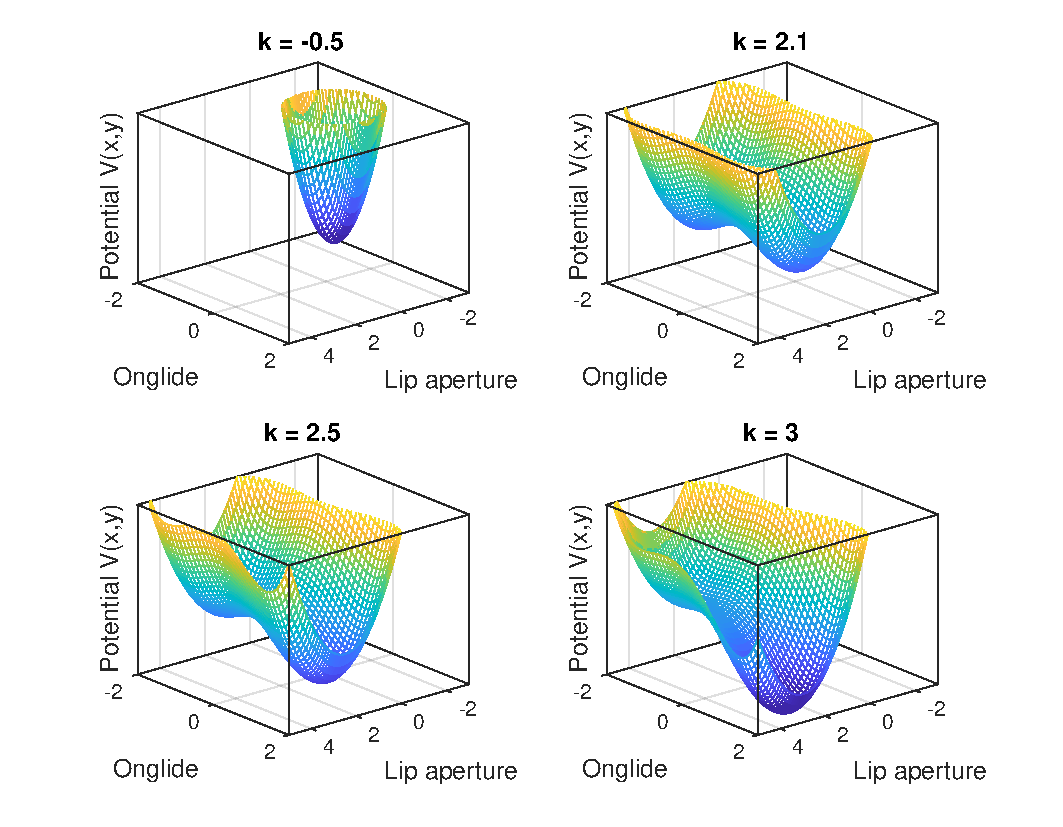
\includegraphics[width=\textwidth]{figures/ch7/3d_landscapes1.pdf}
\caption[Attractor landscapes defined by the dimensions tonal onglide and lip aperture for background, broad, narrow and contrastive focus.]{Attractor landscapes defined by the dimensions tonal onglide and lip aperture for $k$ values modelling background (top left), broad (top right), narrow (bottom left) and contrastive focus (bottom right).}
\label{fig:3d_landscapes1}
\end{figure}

\begin{figure}
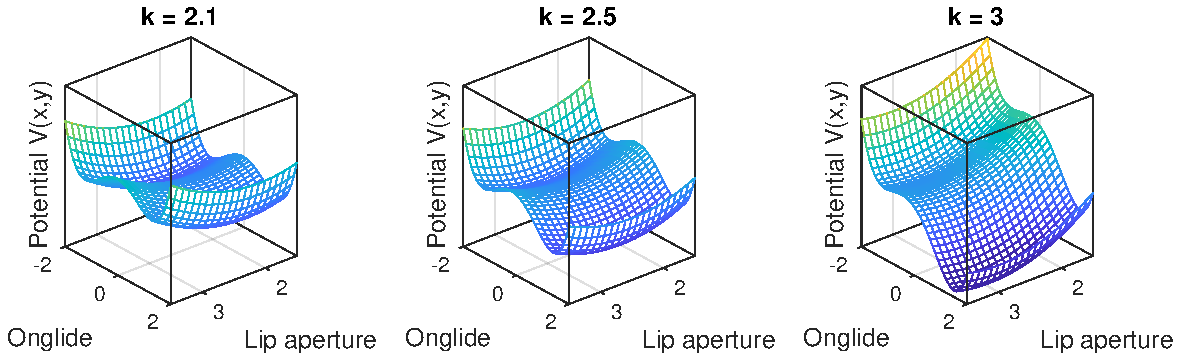
\includegraphics[width=\textwidth]{figures/ch7/3d_landscapes2.pdf}
\caption[Attractor landscapes defined by the dimensions tonal onglide and lip aperture for broad, narrow and contrastive focus.]{Attractor landscapes defined by the dimensions tonal onglide and lip aperture for $k$ values modelling broad (left), narrow (centre) and contrastive focus (right).}
\label{fig:3d_landscapes2}
\end{figure}

The probability density function of this non-deterministic dynamical system can be found as a stationary solution to the Fokker-Planck equation for the system \citep{Haken1977, GafosBenus2006}. In Figure \ref{fig:3d_probs1} and Figure \ref{fig:3d_probs2}, the graphs of probability functions are given for the system with two dimensions from two perspectives. They reveal the pattern described above for the attractor landscapes with a change from a single peak to two almost equal peaks from $k = -0.5$ to $k = 2.1$ (background to broad focus), and a strengthening of the right peak from $k = 2.1$ to $k = 2.5$ (broad focus to narrow focus) and from $k = 2.5$ to $k = 3.0$ (narrow focus to contrastive focus). 

\begin{figure}
	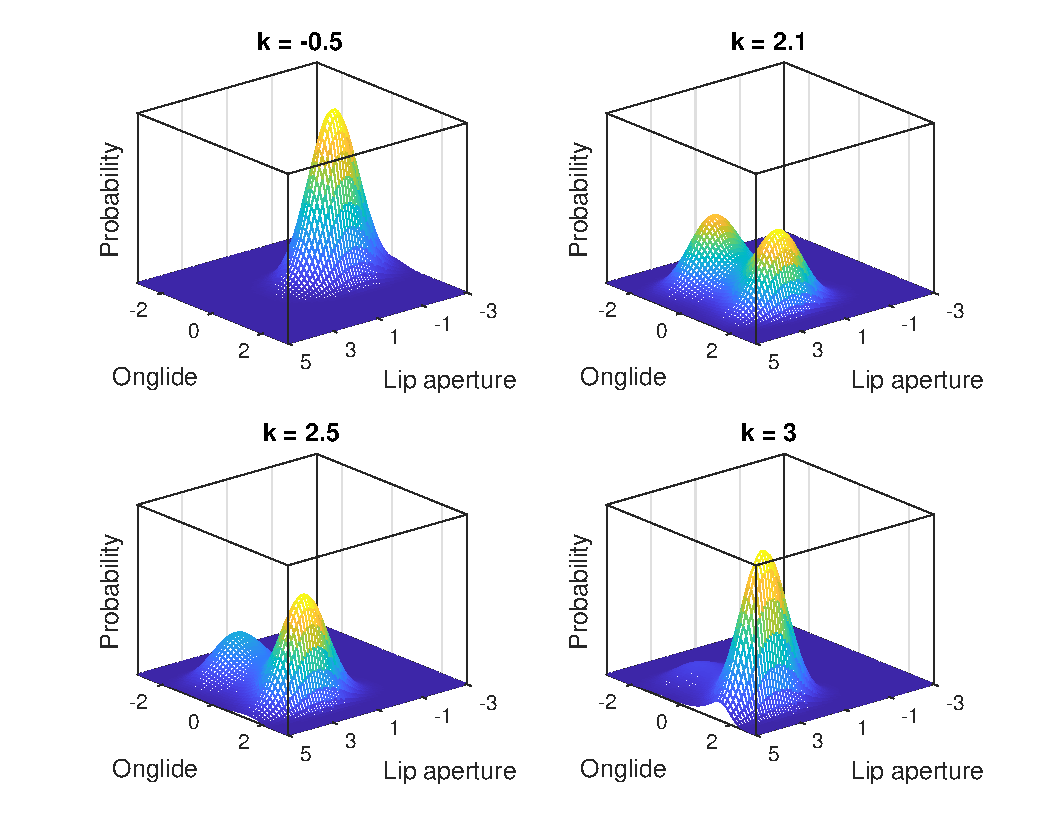
\includegraphics[width=\textwidth]{figures/ch7/probabilities1.pdf}
	\caption[Probability density functions for the system with the $k$ values modelling background, broad, narrow and contrastive focus -- perspective 1.]{Probability density functions for the system with the $k$ values modelling background (top left), broad (top right), narrow (bottom left) and contrastive focus (bottom right) -- perspective 1.}
	\label{fig:3d_probs1}
\end{figure}

The outlined model can be extended by adding an unrestricted number of dimensions, for example the vertical and horizontal tongue body position. Their shape may resemble the shape of the lip aperture dimension. Since the modifications in these parameters go in the opposite direction, the part added to the potential would be minimally different (i.e. $\frac{(z+k)^2}{2}$ instead of $\frac{(z-k)^2}{2}$, where $z$ denotes the state of the tongue position). Most of the results presented above make it plausible to think of these dimensions as being modulated by the same control parameter. The horizontal tongue position of the vowel /a/, however, does not fit in this picture.



\begin{figure}[t]
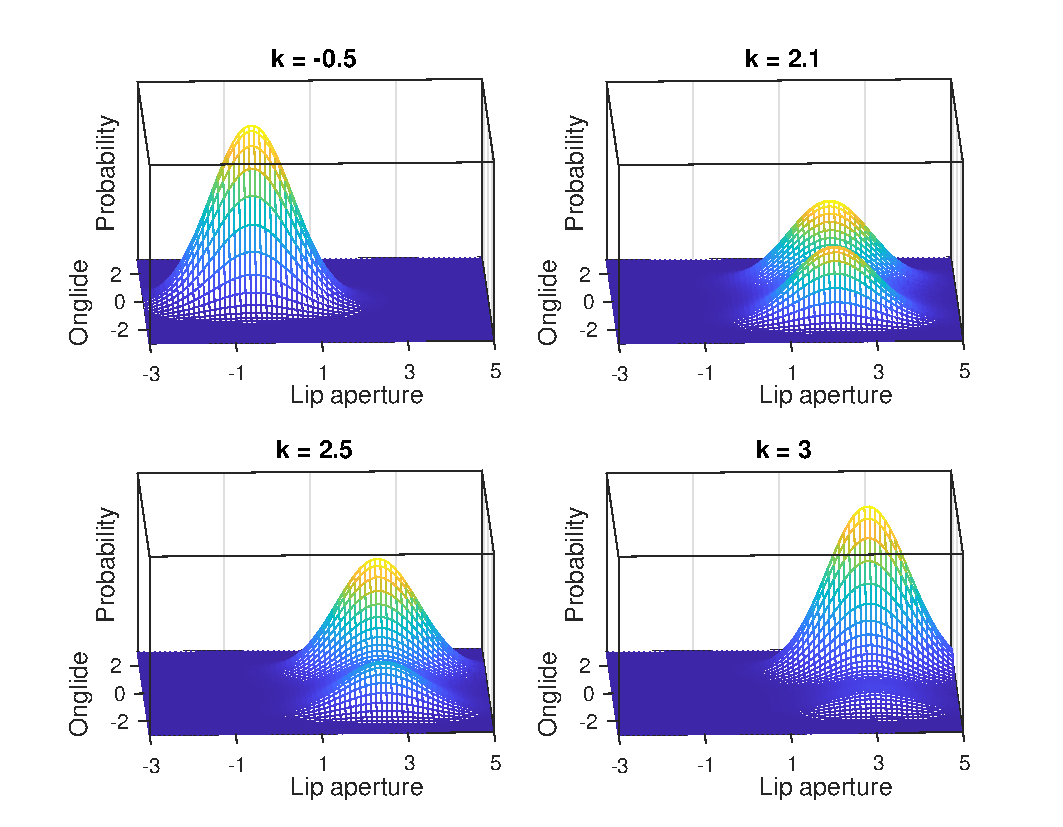
\includegraphics[width=\textwidth]{figures/ch7/probabilities2.pdf}
\caption[Probability density functions for the system with the $k$ values modelling background, broad, narrow and contrastive focus -- perspective 2.]{Probability density functions for the system with the $k$ values modelling background (top left), broad (top right), narrow (bottom left) and contrastive focus (bottom right) -- perspective 2.}
\label{fig:3d_probs2}
\end{figure}

\section{Summary}

This chapter has dealt with the completion of the picture drawn by Chapter \ref{chapter_onglide_modelling} on prosodic marking of focus in German. Tonal and articulatory data of 27 native speakers were presented. The analysis showed that the background condition is characterised by a stretch of flat F0 on and around the target word since no accent is placed on the target word in this condition. The tonal onglide model was extended to be able to capture the change from these flat F0 stretches to falling and rising accents as the result of a bifurcation in the system. 

Furthermore, the examination of the articulatory data revealed that lip aperture and tongue body position are modulated as a means of increasing prosodic prominence continuously through the focus types. This implies that the kinematic parameters are modified from unaccented to accented (background to broad focus) but also from broad to narrow focus and from narrow to contrastive focus. The latter finding is important because it shows that prosody-induced modifications go beyond the categorical notion of accentuation and are used to signal prosodic prominence directly. Emphasising the importance of a multi-dimensional perspective on prosody, a model was sketched that ties the tonal and articulatory dimensions together (and is open to extension to an unrestricted number of dimensions). A key feature of this model is that the dimensions are modulated by the same control parameter.

To conclude, this chapter concentrated on the idea of integration in a two-fold manner: First, a full model of tonal onglide modifications was proposed that is able to capture categorical (accentuation \emph{and} accent types) and continuous aspects of intonation. Second, multiple dimensions were tied together with a joint control parameter in  a dynamical approach.
